\documentclass[11pt]{article}

\usepackage[utf8]{inputenc}
\usepackage[portuges]{babel}
\usepackage{indentfirst}
\usepackage{natbib}
\usepackage{graphicx}
\usepackage{adjustbox}
\usepackage{float}
\usepackage{geometry}
 \geometry{
    a4paper,
    total={130mm,227mm},
    left=30mm,
    right=30mm,
    top=20mm,
    bottom=20mm
}
\setlength\abovecaptionskip{-2pt}
 
\renewcommand{\contentsname}{Índice}

\begin{document}

\begin{titlepage}
    \begin{center}
        
\includegraphics[width=0.3\textwidth]{images/capa/EscolaEngenhariaUM.jpeg}
    
        \vspace{1cm}
        
        \textbf{\LARGE Comunicações por Computador}
    
        \vspace{0.5cm}
        \textbf{\Large Trabalho Prático 3}

        \vspace{1.3cm}
        
        \textbf{\large Luís Pedro Oliveira de Castro Vieira A89601 \\
        José Pedro de Castro Ferreira A89572 \\
        Luís Enes Sousa A89597}

        \vspace{1.5cm}
        \begin{figure}[hbt!]
            \minipage{0.32\textwidth}
                \frame{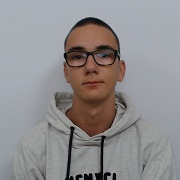
\includegraphics[width=\linewidth]{images/capa/massini.jpg}}
                \centering
                \captionsetup{A89601}
            \endminipage\hfill
            \minipage{0.32\textwidth}
                \frame{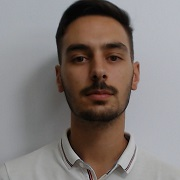
\includegraphics[width=\linewidth]{images/capa/8free.jpg}}
                \centering
                \captionsetup{A89572}
            \endminipage\hfill
            \minipage{0.32\textwidth}
                \frame{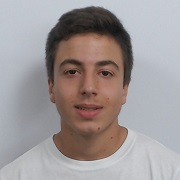
\includegraphics[width=\linewidth]{images/capa/80.jpeg}}
                \centering
                \captionsetup{A89597}
            \endminipage
        \end{figure}
        
       \vspace{8cm}
        
        7 de maio de 2021
        
    \end{center}
\end{titlepage}

\tableofcontents
\thispagestyle{empty}
\cleardoublepage

\setcounter{page}{1}

\section{Parte I}
%-----------------------------------------------------------------%
\subsection{Questões e Respostas}
\vspace{0.5cm}


%-----------------------------------------------------------------%
\subsubsection{Pergunta A}

\textbf{Qual o conteúdo do ficheiro /etc/resolv.conf e para que serve essa informação?}

\par O ficheiro \textit{/etc/resolv.conf} contém informação sobre o nome do servidor DNS local e respetivos IPs para os servidores associados. Esta infomração é variável, uma vez que depende da rede em que o host se encontra. De notar que, quando um utilizador quer aceder a um domínio, o nome do servidor é o primeiro a ser interrogado, procurando pelo mesmo nos registos.

\begin{figure}[!htb]
    \centering
    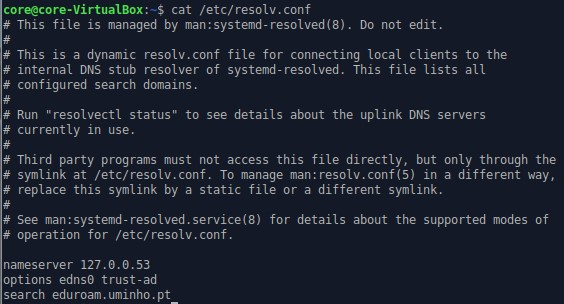
\includegraphics[width=0.8\textwidth]{images/Parte1/p1_a.jpg}
    \caption{Conteúdo do ficheiro /etc/resolv.conf}
    \label{fig:etc/conf}
\end{figure}

%-----------------------------------------------------------------%
\subsubsection{Pergunta B}

\textbf{Os servidores www.uminho.pt. e www.ubuntu.com. têm endereços IPv6? Se sim, quais?}

\par Apenas o servidor www.ubuntu.com possui endereços IPv6, sendo eles:
\begin{itemize}
    \item \textbf{www.ubuntu.com} - 2001:67c:1360:8001::2c
    \item \textbf{www.ubuntu.com} - 2001:67c:1360:8001::2b
\end{itemize}

\begin{figure}[!htb]
    \centering
    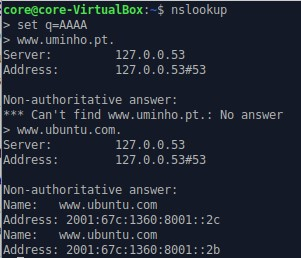
\includegraphics[width=.4\textwidth]{images/Parte1/p1_b2.jpg}
    \caption{Endereços IPv6 do servidor www.ubuntu.com}
    \label{fig:ipv6ubuntu}
\end{figure}

\begin{figure}[!htb]
    \centering
    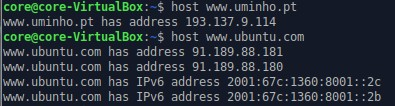
\includegraphics[width=.6\textwidth]{images/Parte1/p1_b.jpg}
    \caption{Endereços IPv6 do servidor www.uminho.pt}
    \label{fig:ipv6ubuntu}
\end{figure}



%-----------------------------------------------------------------%
\subsubsection{Pergunta C}

\textbf{Quais os servidores de nomes definidos para os domínios: “sapo.pt.”, “pt.” e “.”?}

\par Para o domnínio \textit{sapo.pt} estão definidos os servidores \textit{ns.sapo.pt}, \textit{ns2.sapo.pt}, \textit{dns01.sapo.pt}, \textit{dns02.sapot.pt}.

\begin{figure}[!htb]
    \centering
    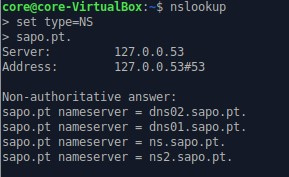
\includegraphics[width=.4\textwidth]{images/Parte1/p1_c1.jpg}
    \caption{Servidores associados ao domínio \textit{'sapo.pt.'}}
    \label{fig:domsapopt}
\end{figure}

\par Já ao domínio \textit{pt.} estão associados 9 servidores, sendo eles:

\begin{figure}[!htb]
    \centering
    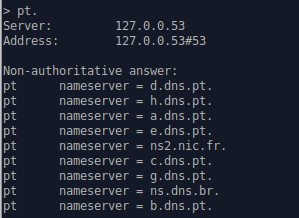
\includegraphics[width=.4\textwidth]{images/Parte1/p1_c2.jpg}
    \caption{Servidores associados ao domínio \textit{'pt.'}}
    \label{fig:dompt}
\end{figure}

\par Por fim, relativamente ao domínio \textit{.} estão definidos 13 servidores.

\begin{figure}[!htb]
    \centering
    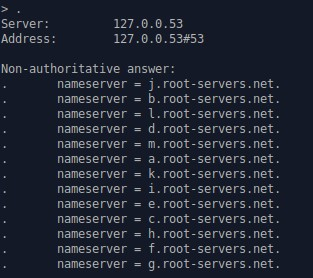
\includegraphics[width=.4\textwidth]{images/Parte1/p1_c3.jpg}
    \caption{Servidores associados ao domínio \textit{'.'}}
    \label{fig:dot}
\end{figure}

%-----------------------------------------------------------------%
\subsubsection{Pergunta D}

\textbf{Existe o domínio open.money.? Será que open.money. é um host ou um domínio?}

\par Sim, o domínio \textit{open.money.} existe, uma vez que existe correspondência para este. No entanto não se trata de um host mas sim de um serviço de email. Isto pode ser comprovado através do uso do comando \textit{host open.money.}, sendo que o resultado do mesmo nos indica que o domínio se trata de um \textit{alias} para um servidor de email.

\begin{figure}[!htb]
    \centering
    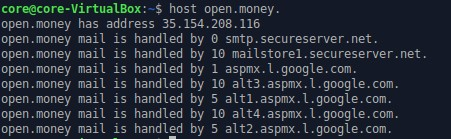
\includegraphics[width=.8\textwidth]{images/Parte1/p1_d.jpg}
    \caption{Execução do comando "host \textit{open.money.}"}
    \label{fig:hostopenmoney}
\end{figure}


%-----------------------------------------------------------------%
\subsubsection{Pergunta E}

\textbf{Qual é o servidor DNS primário definido para o domínio un.org.? Este servidor primário (master) aceita queries recursivas? Porquê?}

\par O servidor DNS primário definido para o domínio \textit{un.org.} é o servidor \textit{ns1.un.org}. Conseguimos confirmar esta informação ao analisar o campo \textit{origin}.

\begin{figure}[!htb]
    \centering
    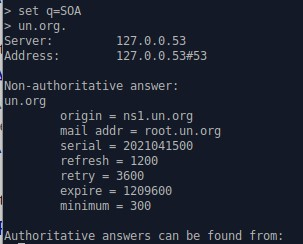
\includegraphics[width=.4\textwidth]{images/Parte1/p1_e.jpg}
    \caption{Execução do comando "nslookup" com uma querie do tipo \textit{SOA} a \textit{un.org.}}
    \label{fig:soaunorg}
\end{figure}

\par Quando executamos o comando \textit{dig un.org.} obtemos as seguintes informações:

\begin{figure}[!htb]
    \centering
    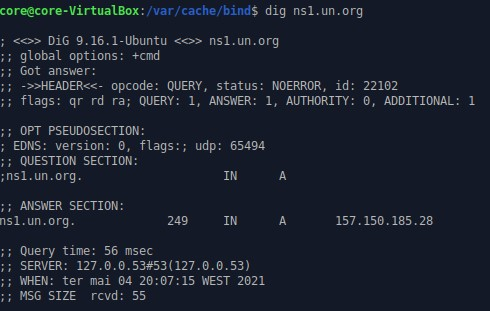
\includegraphics[width=.5\textwidth]{images/Parte1/p1_e2.jpg}
    \caption{Execução do comando "dig \textit{un.org.}"}
    \label{fig:digunorg}
\end{figure}

\par A partir daqui podemos afirmar que este servidor primário aceita queries recursivas uma vez que possui a flag \textit{ra}, 'Recursion Avaiable'.

%-----------------------------------------------------------------%
\subsubsection{Pergunta F}

\textbf{Obtenha uma resposta “autoritativa” para a questão anterior.}

\par Com o intuito de obter uma resposta "autoritativa", executamos o comando "nslookup" com uma query do tipo \textit{SOA}, obtendo o seguinte resultado:

\begin{figure}[!htb]
    \centering
    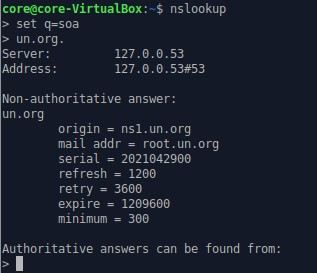
\includegraphics[width=.5\textwidth]{images/Parte1/p1_f1.jpg}
    \caption{Comando "nslookup" com uma query do tipo SOA a "un.org."}
    \label{fig:unSOA}
\end{figure}

\par O passo seguinte seria questionar os servidores autoritativos obtidos, que sabemos ser, pelo menos um, \textit{ns1.un.org}, executando "server ns1.un.org" dentro do "nslookup" e procurando novamente por "un.org". No entanto devido às medidas de segurança da rede, não é possível realizar o mesmo pois estaria a pôr em risco os servidores existentes.

\par O expectado seria que, ao questionar novamente por "un.org" tendo como servidor "ns1.un.org" obtivéssemos uma resposta do tipo \textit{"connection timed out"} uma vez que apenas um servidor local permite responder de forma recursiva ao cliente.

%-----------------------------------------------------------------%
\subsubsection{Pergunta G}

\textbf{Onde são entregues as mensagens de correio eletrónico dirigidas a presidency@eu.eu ou presidencia@2021portugal.eu?}

\par Para obter a informação acerca do destino das mensagens de correio eletrónico temos que executar os comandos descritos abaixo:

\begin{figure}[!htb]
    \centering
    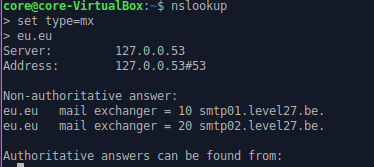
\includegraphics[width=.5\textwidth]{images/Parte1/p1_g1.PNG}
    \caption{Comando "nslookup" como uma query do tipo MX}
    \label{fig:emailMX}
\end{figure}

\begin{figure}[!htb]
    \centering
    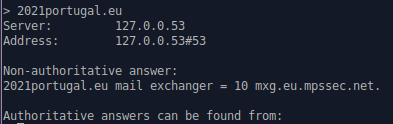
\includegraphics[width=.5\textwidth]{images/Parte1/p1_g2.PNG}
    \caption{Comando "nslookup" como uma query do tipo MX}
    \label{fig:emailMX}
\end{figure}

\par Assim sendo, sabemos que as mensagens enviadas a \textit{presidencia@2021portugal.eu.} irão ser entregues em \textit{mxg.eu.mpssec.net.}.

\par Já as mensagens enviadas para \textit{presidency@eu.eu} poderão ser entregues em duas opções diferentes: \textit{smtp01.level27.be.} ou \textit{smtp02.level27.be.}. No entanto, o primeiro mencionado possui um valor de 10, enquanto que o segundo possui um valor de 20. Isto significa que o primeiro é o servidor prioritário, ou seja, as mensagens serão entregues a este, e só em caso de indisponibilidade serão entregues a \textit{smtp02.level27.be.}

%-----------------------------------------------------------------%
\subsubsection{Pergunta H}

\textbf{Que informação é possível obter, via DNS, acerca de gov.pt?}

\par Executando o comando \textit{"dig dov.pt ANY"} obtivemos o seguinte resultado:

\begin{figure}[!htb]
    \centering
    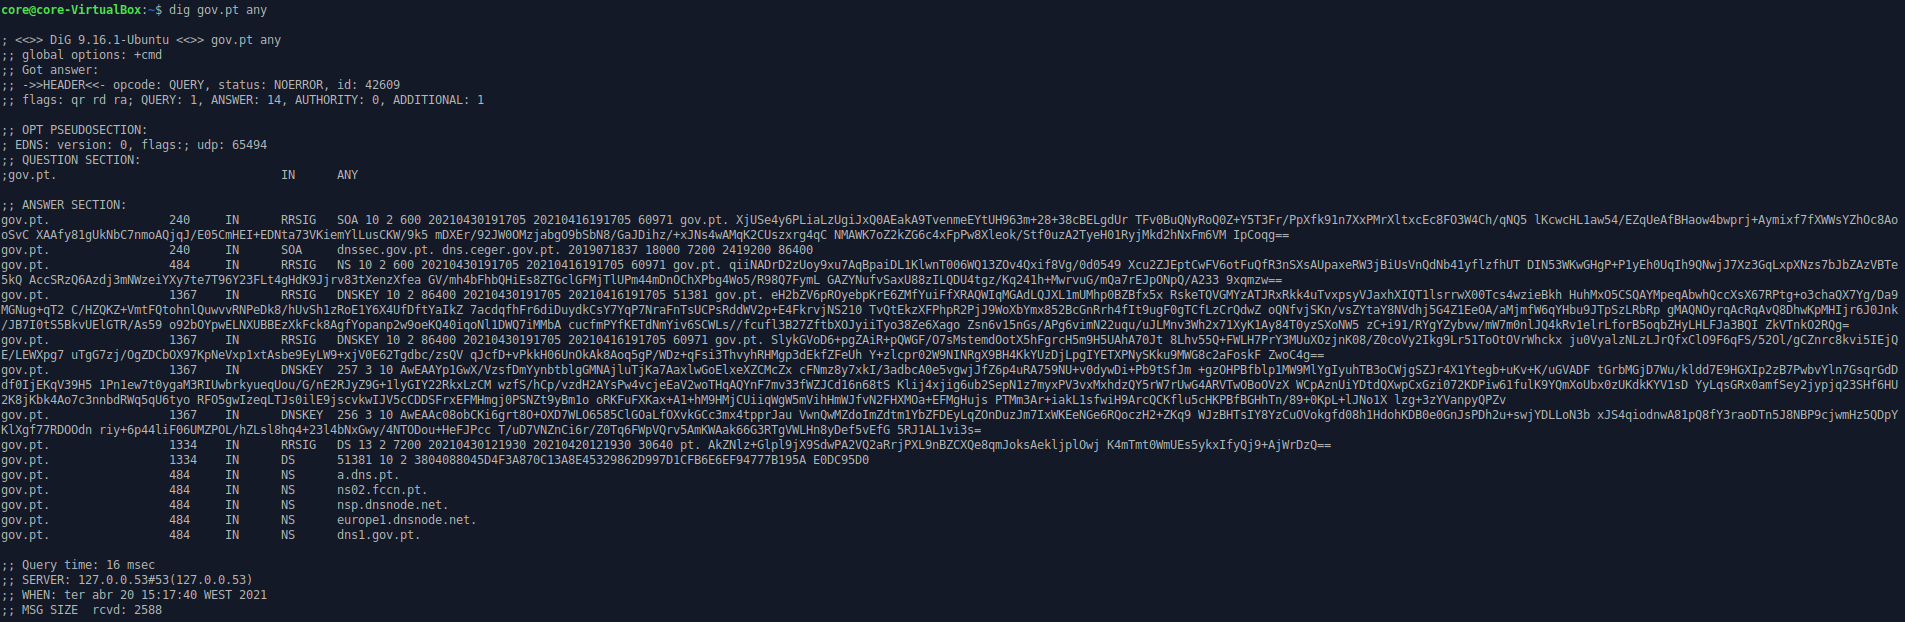
\includegraphics[width=\textwidth]{images/Parte1/p1_h.PNG}
    \caption{Comando \textit{"dig gov.pt ANY"}}
    \label{fig:diggov}
\end{figure}

\par Atentando à secção "Answer Question", podemos encontrar diversas informações acerca de \textit{gov.pt} tais como os servidores associados ao domínio, como por exemplo \textit{dns1.gov.pt.} e \textit{nsp.dnsnode.net.}. Podemos também evidenciar, através da resposta do tipo \textit{SOA}, o seu servidor primário, \textit{dnssec.gov.pt.}, o servidor de email, \textit{dns.ceger.gov.pt.}, e outras informações.

\par Por fim, pode ser ainda encontrada informação sobre registos \textit{RRSIG} e as respetivas keys \textit{DNSKEY} os quais contém um ou mais registos DNS que podem ser acedidos com a chave \textit{DNSKEY}.

%-----------------------------------------------------------------%
\subsubsection{Pergunta I}

\textbf{Consegue interrogar o DNS sobre o endereço IPv6 2001:690:2080:8005::38 usando algum dos clientes DNS? Que informação consegue obter? Supondo que teve problemas com esse endereço, consegue obter um contacto do responsável por esse IPv6?}

\par Através do uso do comando \textit{'nslookup'}, executando uma query do tipo \textit{PTR}, conseguimos interrogar o DNS sobre o endereço IPv6 apresentado, através de \textit{reverse mapping}, conseguindo assim obter o domínio ao qual o endereço está associado.

\begin{figure}[!htb]
    \centering
    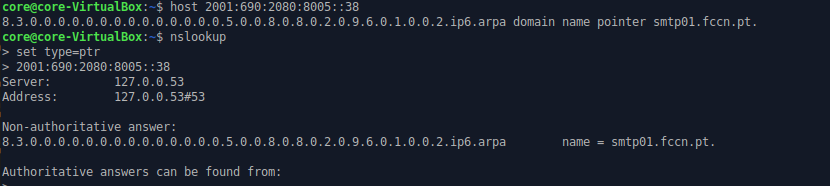
\includegraphics[width=.8\textwidth]{images/Parte1/p1_i1.PNG}
    \caption{Comando \textit{"nslookup"} com uma query do tipo PTR}
    \label{fig:nsIPV6PTR}
\end{figure}

\par Podemos então concluir que o domínio ao qual o endereço IPv6 2001:690:2080:8005::38 se encontra associado é \textit{ffcn.pt.}. Fazendo uso desta informação e realizando agora uma query do tipo \textit{SOA} conseguimos obter o contacto dos responsáveis por esse mesmo endereço.

\begin{figure}
    \centering
    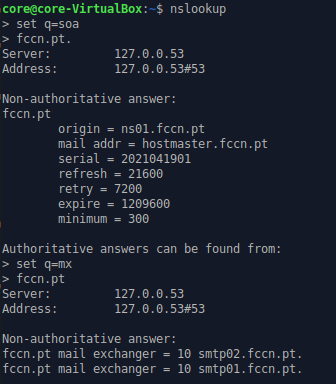
\includegraphics[width=.4\textwidth]{images/Parte1/p1_i2.PNG}
    \caption{Comando \textit{"nslookup"} com uma query do tipo \textit{SOA}}
    \label{fig:nsIPV6SOA}
\end{figure}

\par Avaliando então o resultado obtido, podemos concluir que o responsável pelo endereço IPv6 apresentado no enunciado é \textit{ns01.ffcn.pt}.

%-----------------------------------------------------------------%
\subsubsection{Pergunta J}

\textbf{Os secundários usam um mecanismo designado por “Transferência de zona” para se atualizarem automaticamente a partir do primário, usando os parâmetros definidos no Record do tipo SOA do domínio. Descreve sucintamente esse mecanismo com base num exemplo concreto (ex: di.uminho.pt ou o domínio cc.pt que vai ser criado na topologia virtual).}

\par A "transferência de zona" DNS é um tipo de transação de DNS, um dos muitos mecanimos disponíveis para os administradores replicarem bases de dados DNS num conjunto de servidores DNS secundários. Uma transferência de zona usa o TCP para transporte e assume a forma de uma transação cliente-servidor.

\par Isto é, um cliente solicita uma transferência de dados de um servidor primário para um secundário, sendo a parte da base de dados replicada designada por zona.

\par Através dos parâmetros definidos no registo do tipo SOA, e fazendo uso do domínio cc.pt criado na topologia virtual, podemos visualizar as seguintes informações:

\begin{figure}[!htb]
    \centering
    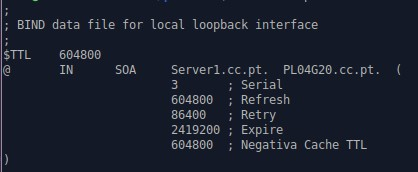
\includegraphics[width=.7\textwidth]{images/Parte1/p1_j.jpg}
    \caption{Conteúdo do registo do tipo SOA \textit{bd.cc.pt}}
    \label{fig:dbccpt}
\end{figure}

\begin{itemize}
    \item \textbf{Serial} - Corresponde ao número de série da zona. Se o servidor secundário associado a este verificar uma alteração neste, assume que a zona está desatualizada e inicia-se uma transferência de zona.
    \item \textbf{Refresh} - Número de segundos após o qual o servidor secundário contactará o servidor primário para atualizar informações, de modo a detetar possíveis alterações na zona.
    \item \textbf{Retry} - Corresponde ao número de segundos que o servidor secundário deve esperar após uma falha para se reconectar novamente ao servidor primário, sendo que este deve ser sempre inferior ao valor de \textit{refresh}.
    \item \textbf{Expire} - Número de segundos após o qual o servidor secundário deve parar de fazer solicitações para a zona específica, caso o servidor primário não responda. Este valor deve ser superior à soma do valor do \textit{refresh} e do \textit{retry}.
\end{itemize}

\par Em suma, o servidor secundário deverá contactar o primário para se atualizar após 604800 segundos terem passado; deve esperar 86400 segundos até poder tentar uma nova conexão com o servidor primário após ter falhado inicialmente; caso o servidor primário não responda, até 2419200 segundos depois, o servidor secundário deixa de tentar conectar-se.



%-----------------------------------------------------------------%
\cleardoublepage
\section{Parte II}

\subsection{Domínio CC.PT}

\par Durante a execução de grande parte das instruções presentes no enunciado, limitámo-nos a seguir as mesmas em diversas alturas uma vez que não havia mais alternativas relativamente às mesmas. No entanto houve vezes em que o grupo teve de tomar certas decisões e refletir sobre as mesmas, e estas serão os principais focos de discussão e explicação no presente relatório.

\par A primeira decisão vem no seguimento da instrução presente no enunciado referente ao ficheiro \textit{"named.conf"}. Neste ficámos de incluir as diferentes zonas presentes na topologia core apresentada para o ano de 2021. No entanto no enunciado apenas fazia menção à zona \textit{"cc.pt"} e à zona \textit{"1.1.10.in-addr.arpa}, mas a topologia apresenta 4 redes LAN diferentes, o que levou o grupo a incluir também as zonas de procura inversa para as redes que faltavam, nomeadamente: \textit{"2.2.10.in-addr.arpa"}, \textit{"3.3.10.in-addr.arpa"} e \textit{"4.4.10.in-addr.arpa"}.
\quad O ficheiro ficou assim com 5 zonas.

\par Em cada zona definida no ficheiro "named.conf" tivemos que definir as mesmas com o tipo \textit{master}, uma vez que fazem parte do servidor DNS principal. Tivemos também que adicionar uma cláusula \textit{"allow-transfer \{10.2.2.2;\}"} que permitisse ao servidor secundário transferir e guardar a informação sobre o servidor primário na sua base de dados.

% Incluir print do named.conf

\begin{figure}[!htb]
    \centering
    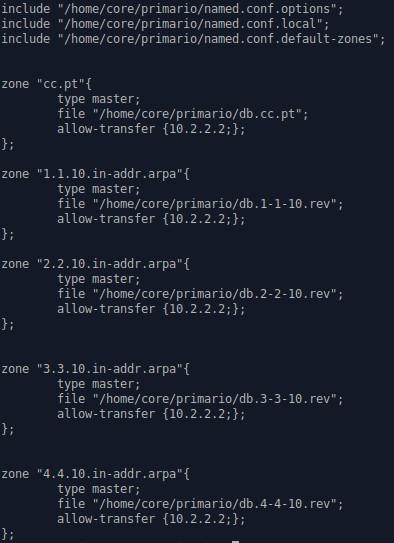
\includegraphics[width=.6\textwidth]{images/Parte2/2_a.jpg}
    \caption{Conteúdo do ficheiro \textit{named.conf}}
    \label{fig:namedconf}
\end{figure}

\par Depois de termos as zonas definidas e criadas segui-se a criação e configuração do ficheiro \textit{"db.cc.pt"}. O primeiro passo neste processo foi a configuração do SOA (Start of Authority), para o qual escolhemos \textit{Server1.cc.pt} para a posição do DNS principal, visto se tratar do servidor principal, e como administrador, como referido no enunciado, estabelecemos que seria \textit{PL04G20.cc.pt}.

\begin{figure}[H]
    \centering
    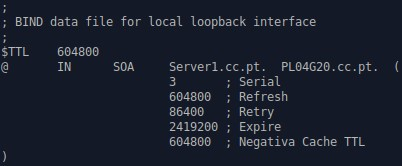
\includegraphics[width=.6\textwidth]{images/Parte2/2_SOA.jpg}
    \caption{Configuração SOA do ficheiro \textit{db.cc.pt}}
    \label{fig:soaCCPT}
\end{figure}

\par Após termos estabelecido o SOA, resta-nos introduzir o resto da informação necessária para o bom funcionamento do nosso servidor DNS. Começámos por introduzir os \textit{nameservers}, nomedamente \textit{Server1} e \textit{Mercurio} fazendo uso da cláusula \textit{NS} e os servidores de email \textit{Server2}, como prioritário, e \textit{Server3.cc.pt} como secundário, como referido no enunciado, desta vez com a cláusula \textit{MX}.

\par De seguida, para todos os elementos inserimos os seus nomes mencionados na topologia bem como o seu endereço IP, fazendo uso da cláusula \textit{A}, resolvendo assim os requisitos Marte.cc.pt, Mercurio.cc.pt e Venus.cc.pt. Adicionamos ainda \textit{alias} para alguns dos elementos como requisitado no enunciado, tais como \textbf{ns} e \textbf{ns2} para os servidores primário e secundário respetivamente.

\par Foi ainda necessário definir os serviços requisitados no enunciado como o servidor web e servidor e-mail, presentes em \textbf{Server2}, e servidor pop e imap, presentes em \textit{Server3}.

\begin{figure}[H]
    \centering
    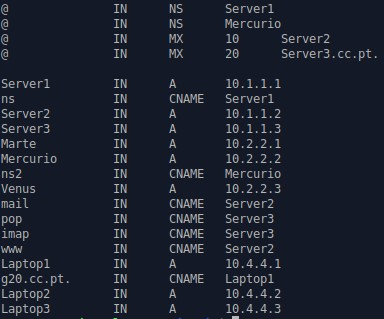
\includegraphics[width=.6\textwidth]{images/Parte2/2_restoCCPT.jpg}
    \caption{Configuração da base de dados cc.pt}
    \label{fig:configCCPT}
\end{figure}

\par Após o término da configuração da base de dados cc.pt, procedemos à configuração dos restantes ficheiros que permitirão a procura inversa. E, embora havendo 4 redes diferentes, o processo é semelhante para todos, acabando por ter a mesma configuração SOA e a adição dos dois \textit{nameservers}: \textit{Server1} e \textit{Mercurio}.

\par Sendo assim, resta-nos apenas introduzir o conhecimento necessário para podermos fazer o \textit{reverse mapping}, o qual fazemos introduzindo o endereço da máquina em questão e o seu nome, acompanhados da cláusula \textit{PTR}.

\begin{figure}[H]
    \centering
    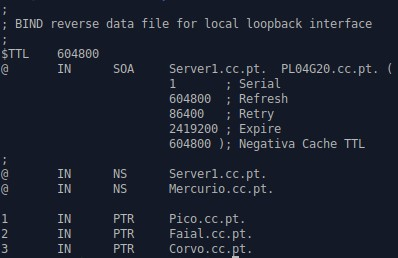
\includegraphics[width=.6\textwidth]{images/Parte2/2_reverseExemplo.jpg}
    \caption{Exemplo do reverse mapping para a rede 10.3.3.0/24}
    \label{fig:rev10330}
\end{figure}

\par Com a conclusão da configuração das bases de dados para os domínios reversos, podemos dar por concluída a configuração do servidor DNS principal.

\par Na configuração do servidor secundário foi apenas necessário alterar o ficheiro \textit{named.conf},
adicionando as zonas existentes no servidor primário com algumas alterações nas cláusulas previamente apresentadas. O \textit{type} que antes era \textit{master} agora passa a ser \textit{slave}, e a cláusula \textit{allow-transfer} foi substituída pela cláusula \textit{masters \{10.1.1.1;\}}, sendo também o path para o ficheiro atualizado.

\begin{figure}[H]
    \centering
    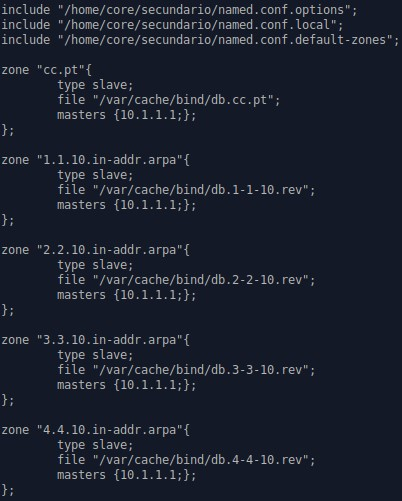
\includegraphics[width=.6\textwidth]{images/Parte2/2_sec.jpg}
    \caption{Configuração do ficheiro \textit{named.conf} do servidor secundário}
    \label{fig:namedsec}
\end{figure}


\clearpage
\section{Conclusão}

\par Tendo terminado o terceiro trabalho prático da Unidade Curricular de Comunicações por Computador, conseguimos afirmar com certezas que fomos capazes de aprofundar em pleno o nosso conhecimento, pondo em prática os conteúdos lecionados nas aulas teóricas.

\par Assim sendo, somos capazes de apresentar como resultado final deste trabalho, ambos os servidores, primário e secundário, funcionais na sua capacidade total. Apesar das dificuldades encontradas durante a resolução do projeto, o grupo conseguiun superá-las e todas as indicações propostas foram completadas com sucesso, apresentando um trabalho consistente e devidamente estruturado.

\end{document}
